\documentclass[xcolor=dvipsnames]{beamer}
\usecolortheme[named=Brown]{structure}
\usetheme{default}
\setbeamertemplate{navigation symbols}{} 
\usepackage{tikz}
\usetikzlibrary{arrows,decorations.pathmorphing,backgrounds,positioning,fit}
\usetikzlibrary{datavisualization.formats.functions}
%     
%Here are some macro's saving time and labour:     
%     
\newcommand{\const}{\mbox{const}}      
\newcommand{\est}{\mbox{{\tiny est}}}      
\newcommand{\im}{\mbox{$\Im \mbox{m}$}}      
\newcommand{\obs}{\mbox{{\tiny obs}}}      
\newcommand{\otherwise}{\mbox{otherwise}}      
\newcommand{\real}{\mbox{$\Re \mbox{e}$}}      
\newcommand{\sign}{\mbox{sign}}      
\newcommand{\sinc}{\mbox{sinc}}      
%
\newcommand{\p}{\mbox{$\partial$}}      
\renewcommand{\d}{\mbox{$\partial$}}      
\newcommand{\w}{\mbox{$\omega$}}      
%
\newcommand{\AAA}{\mbox{\boldmath $A$}}   
\newcommand{\BB}{\mbox{\boldmath $B$}}     
\newcommand{\CC}{\mbox{\boldmath $C$}}     
\newcommand{\DD}{\mbox{\boldmath $D$}}     
\newcommand{\EE}{\mbox{\boldmath $E$}}     
\newcommand{\FF}{\mbox{\boldmath $F$}}   
\newcommand{\GG}{\mbox{\boldmath $G$}}   
\newcommand{\HH}{\mbox{\boldmath $H$}}   
\newcommand{\II}{\mbox{\boldmath $I$}}   
\newcommand{\JJ}{\mbox{\boldmath $J$}}   
\newcommand{\KK}{\mbox{\boldmath $K$}}   
\newcommand{\LL}{\mbox{\boldmath $L$}}   
\newcommand{\MM}{\mbox{\boldmath $M$}}   
\newcommand{\NN}{\mbox{\boldmath $N$}}   
\newcommand{\OO}{\mbox{\boldmath $O$}}   
\newcommand{\PP}{\mbox{\boldmath $P$}}   
\newcommand{\QQ}{\mbox{\boldmath $Q$}}   
\newcommand{\RR}{\mbox{\boldmath $R$}}   
\newcommand{\SSS}{\mbox{\boldmath $S$}}   
\newcommand{\TT}{\mbox{\boldmath $T$}}   
\newcommand{\UU}{\mbox{\boldmath $U$}}   
\newcommand{\VV}{\mbox{\boldmath $V$}}   
\newcommand{\WW}{\mbox{\boldmath $W$}}   
\newcommand{\XX}{\mbox{\boldmath $X$}}   
\newcommand{\YY}{\mbox{\boldmath $Y$}}   
\newcommand{\ZZ}{\mbox{\boldmath $Z$}}   
%
%\newcommand{\aaa}{\mbox{\boldmath $a$}}     
\newcommand{\bb}{\mbox{\boldmath $b$}}     
\newcommand{\cc}{\mbox{\boldmath $c$}}     
\newcommand{\dd}{\mbox{\boldmath $d$}}     
\newcommand{\ee}{\mbox{\boldmath $e$}}   
\newcommand{\ff}{\mbox{\boldmath $f$}}   
%\newcommand{\ggg}{\mbox{\boldmath $g$}}   
\newcommand{\hh}{\mbox{\boldmath $h$}}   
\newcommand{\ii}{\mbox{\boldmath $i$}}   
\newcommand{\jj}{\mbox{\boldmath $j$}}   
\newcommand{\kk}{\mbox{\boldmath $k$}}   
%\newcommand{\lll}{\mbox{\boldmath $l$}}   
\newcommand{\mm}{\mbox{\boldmath $m$}}   
\newcommand{\nn}{\mbox{\boldmath $n$}}   
\newcommand{\pp}{\mbox{\boldmath $p$}}   
\newcommand{\qq}{\mbox{\boldmath $q$}}   
\newcommand{\rr}{\mbox{\boldmath $r$}}   
%\newcommand{\sss}{\mbox{\boldmath $s$}}   
%\newcommand{\ttt}{\mbox{\boldmath $t$}}   
\newcommand{\uu}{\mbox{\boldmath $u$}}   
\newcommand{\vv}{\mbox{\boldmath $v$}}   
\newcommand{\ww}{\mbox{\boldmath $w$}}   
\newcommand{\xx}{\mbox{\boldmath $x$}}   
\newcommand{\yy}{\mbox{\boldmath $y$}}   
\newcommand{\zz}{\mbox{\boldmath $z$}}   
%
\newcommand{\balpha}{\mbox{\boldmath $\alpha$}}     
\newcommand{\bpsi}{\mbox{\boldmath $\psi$}}     
\newcommand{\bphi}{\mbox{\boldmath $\phi$}}     
\newcommand{\bbeta}{\mbox{\boldmath $\beta$}}     
\newcommand{\btheta}{\mbox{\boldmath $\theta$}}     
\newcommand{\bdelta}{\mbox{\boldmath $\delta$}}     
\newcommand{\bgamma}{\mbox{\boldmath $d$}}     
\newcommand{\bGamma}{\mbox{\boldmath $\Gamma$}}     
\newcommand{\bLambda}{\mbox{\boldmath $\Lambda$}}     
\newcommand{\bmu}{\mbox{\boldmath $\mu$}}     
\newcommand{\bnabla}{\mbox{\boldmath $\nabla$}}     
\newcommand{\brho}{\mbox{\boldmath $\rho$}}     
\newcommand{\bSigma}{\mbox{\boldmath $\Sigma$}}     
\newcommand{\bsigma}{\mbox{\boldmath $\sigma$}}     
\newcommand{\bxi}{\mbox{\boldmath $\xi$}}     
\newcommand{\bepsilon}{\mbox{\boldmath $\epsilon$}}     
\newcommand{\blambda}{\mbox{\boldmath $\lambda$}}     
\newcommand{\BLambda}{\mbox{\boldmath $\Lambda$}}     
%-------------------------------------%
%  \Appendix - a new appendix command %
%-------------------------------------%
%The appendix command is used as in
% \Appendix{A}{The wave equation as a matrix equation}
\newcommand {\Appendix}[1]{
              \section*{APPENDIX #1}
              \setcounter{equation}{0}
              \renewcommand{\theequation} 
              {A-\arabic{equation}}}
\newcommand {\Appendices}[2]{
              \section*{APPENDIX #1: #2 }
              \setcounter{equation}{0}
              \renewcommand{\theequation} 
              {#1-\arabic{equation}}}
%------------------------------------%
%    \aref - a new cite command.     % 
%------------------------------------%
\newcommand{\aref}[2]{\nocite{#1}#2} 
%----------------------------------------
%\eqref -an equation reference command
%----------------------------------------
%\newcommand{\eqref}[1]{(\ref{#1})}
%\newcommand{\eqref}[1]{\ref{#1}}

\usepackage{epsfig}
\usepackage{natbib}
\begin{document}
%\setbeamercolor{titlelike}{fg=gray,bg=white}
%\setbeamercolor{itemize item}{fg=gray,bg=white}
%\setbeamercolor{enumerate item}{fg=gray,bg=white}
%\setbeamercolor{block title}{fg=black,bg=white}
%==============================================
\title{True amplitude cross-correlation imaging condition for Reverse Time Migration}
\author{B. Arntsen and E. B. Raknes}
\institute[NTNU]{
  NTNU\\
  Department of Geoscience and petroleum \\
  \texttt{borge.arntsen@ntnu.no}
}
\date{EGU General Assembly 2017}
\begin{frame}
 \titlepage
\end{frame}
%==============================================
%-----------------------------------------
\begin{frame}{Overview}
%-----------------------------------------
\begin{enumerate}
  \item Introduction
  \item True Amplitude Imaging condition
  \item Numerical examples
  \item Conclusions
\end{enumerate}
\end{frame}
%-----------------------------------------
\begin{frame}{Introduction}
%-----------------------------------------
\begin{enumerate}
   \item Reverse time migration is used both on
         exploration and global scale
   \item The so called imaging condition is crucial for
         the resolution and accuracy of the image
   \item The standard imaging condition in use today can
         be easily modified to give better accuracy and
         resolution 
   \item The modification also gives reflectivity with
         correct amplitudes
\end{enumerate}
\end{frame}
%-----------------------------------------
\begin{frame}{Imaging condition I}
%-----------------------------------------
\begin{figure}
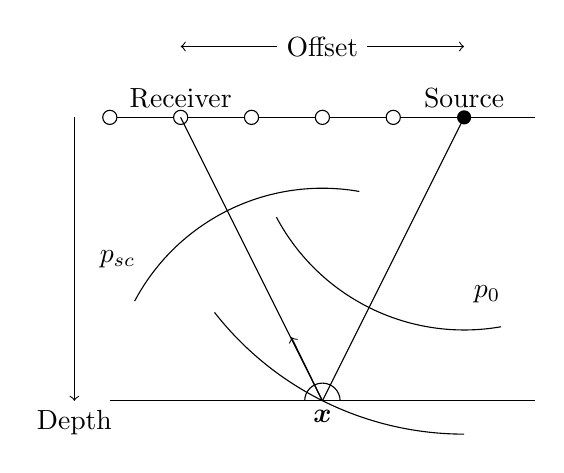
\begin{tikzpicture}[scale=0.9]
  \draw[->] (-0.5,4.0) -- (-0.5,0.0) node[below]{Depth} ;
  \draw[<->] (1.0,5.0) -- node[fill=white]{Offset} (5.0,5.0); 
  \draw (0.0,0.0) -- (6.0,0.0) ;
  \draw (0.0,4.0) -- (6.0,4.0) ;
  \fill (5.0,4.0) node[above]{Source} circle (0.1) ;
  \fill[white] (0.0,4.0) circle (0.1) ;
  \draw (0.0,4.0) circle (0.1) ;
  \fill[white](1.0,4.0) circle (0.1) ;
  \draw (1.0,4.0) node[above]{Receiver}circle (0.1) ;
  \fill[white] (2.0,4.0) circle (0.1) ;
  \draw (2.0,4.0) circle (0.1) ;
  \fill[white] (3.0,4.0) circle (0.1) ;
  \draw (3.0,4.0) circle (0.1) ;
  \fill[white] (4.0,4.0) circle (0.1) ;
  \draw (4.0,4.0) circle (0.1) ;
  \draw (5.0,4.0) -- (3.0,0.0) ;
  \draw (3.0,0.0) -- (1.0,4.0) ;
% Upgoing wave circle
  \draw (3,0) +(80:3) arc(80:152:3);
  \draw (3,0) +(0:0.25) arc(0:180:0.25);
  \draw (5,4) +(-80:3) arc(-80:-152:3);
  \draw (5,4) +(-90:4.47) arc(-90:-142:4.47);
  \draw (5.0,1.5) node[right]{$p_0$};
  \draw (0.5,2.0) node[left]{$p_{sc}$};
  \draw (3,0) node[below]{$\xx$};
  %\draw (3.4,0.125) node[below]{$\xx'$};
  \draw[->] (3,0)-- +(116:1);
\end{tikzpicture}
%\label{fig:si-1}
\end{figure}
$p_{sc}$: Scattereded wavefield (data)\\
$p_{0}$: Modeled wavefield\\
$\xx$: Spatial position
\end{frame}
%-----------------------------------------
\begin{frame}{Imaging condition II}
%-----------------------------------------
\begin{figure}
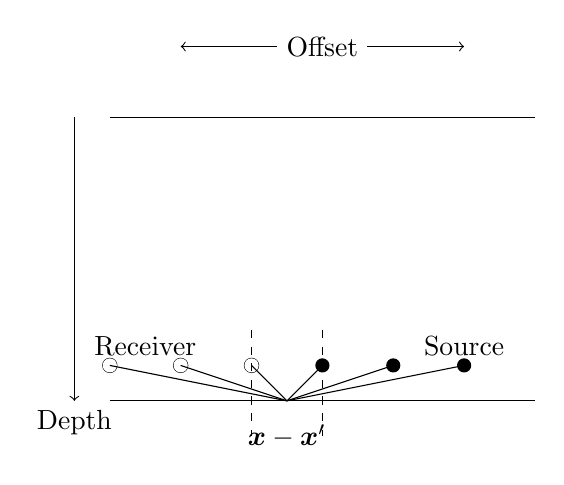
\begin{tikzpicture}[scale=0.9]
   \draw[->] (-0.5,4.0) -- (-0.5,0.0) node[below]{Depth} ;      %Depth axis 
   \draw[<->] (1.0,5.0) -- node[fill=white]{Offset} (5.0,5.0);  %Offset axis  
  \draw (0.0,4.0) -- (6.0,4.0) ;                               % Boundary at top
  \draw (0.0,0.0) -- (6.0,0.0) ;                               % Boundary at depth

  \fill (3.0,0.5) node[above]{} circle (0.1) ;           % Draw source
  \fill (4.0,0.5) node[above]{} circle (0.1) ;           % Draw source
  \fill (5.0,0.5) node[above]{Source} circle (0.1) ;     % Draw source text

  \draw (2.0,0.5) circle (0.1) ;             %Draw receiver
  \fill[white] (2.0,0.5) circle (0.1) ;

  \draw (1.0,0.5) circle (0.1) ;             %Draw receiver
  \fill[white] (1.0,0.5) circle (0.1) ;

  \draw (0.0,0.5) circle (0.1) ;             %Draw receiver
  \fill[white] (0.0,0.5) circle (0.1) ;
  \draw (0.5,0.5) node[above]{Receiver} ;    %Draw receiver text 

  \draw (3.0,0.5) -- (2.5,0.0);              % Draw ray from source to midpoint
  \draw (4.0,0.5) -- (2.5,0.0);              % Draw ray from source to midpoint
  \draw (5.0,0.5) -- (2.5,0.0);              % Draw ray from source to midpoint

  \draw (2.0,0.5) -- (2.5,0.0);              % Draw ray from receiver to midpoint
  \draw (1.0,0.5) -- (2.5,0.0);              % Draw ray from receiver to midpoint
  \draw (0.0,0.5) -- (2.5,0.0);              % Draw ray from receiver to midpoint

  \draw[dashed] (2.0,1.0) -- (2.0,-0.5);     %Draw vertical dashed line
  \draw[dashed] (3.0,1.0) -- (3.0,-0.5);     %Draw vertical dashed line
  \draw (2.5,-0.5) node {$\xx-\xx'$};           % Draw equation

\end{tikzpicture}
%\label{fig:si-1}

$\xx$: Virtual receiver\\
$\xx'$: Virtual source
\end{figure}
\end{frame}
%-----------------------------------------
\begin{frame}{Imaging condition III}
%-----------------------------------------
\begin{figure}
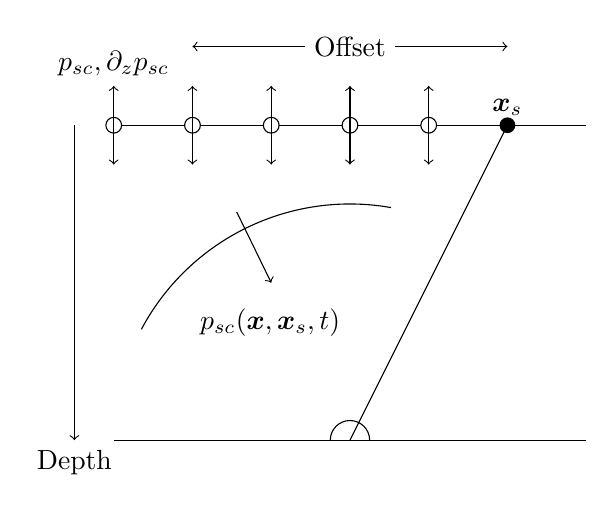
\begin{tikzpicture}[scale=1.0]
  \draw[->] (-0.5,4.0) -- (-0.5,0.0) node[below]{Depth} ;     %Draw Depth axis
  \draw[<->] (1.0,5.0) -- node[fill=white]{Offset} (5.0,5.0); %Draw offset axis 
  \draw (0.0,0.0) -- (6.0,0.0) ;  %Top boundary
  \draw (0.0,4.0) -- (6.0,4.0) ;  %Bottom boundary

  \fill (5.0,4.0) node[above]{$\xx_s$} circle (0.1) ; % Draw source

  \fill[white] (0.0,4.0) circle (0.1) ; %Draw receiver
  \draw (0.0,4.0) circle (0.1) ;
  \draw[->] (0.0,4.0) -- (0.0,4.5);
  \draw[->] (0.0,4.0) -- (0.0,3.5);
  \draw (0.0,4.5) node[above]{$p_{sc},\partial_z p_{sc}$};
  

  \fill[white](1.0,4.0) circle (0.1) ;
  \draw (1.0,4.0) node[above]{} circle (0.1) ;
  \draw[->] (1.0,4.0) -- (1.0,4.5);
  \draw[->] (1.0,4.0) -- (1.0,3.5);

  \fill[white] (2.0,4.0) circle (0.1) ;
  \draw (2.0,4.0) circle (0.1) ;
  \draw[->] (2.0,4.0) -- (2.0,4.5);
  \draw[->] (2.0,4.0) -- (2.0,3.5);

  \fill[white] (3.0,4.0) circle (0.1) ;
  \draw (3.0,4.0) circle (0.1) ;
  \draw[->] (3.0,4.0) -- (3.0,4.5);
  \draw[->] (3.0,4.0) -- (3.0,3.5);

  \fill[white] (4.0,4.0) circle (0.1) ;
  \draw (4.0,4.0) circle (0.1) ;
  \draw[->] (4.0,4.0) -- (4.0,4.5);
  \draw[->] (4.0,4.0) -- (4.0,3.5);

  \draw[<-] (2,2)-- +(116:1);
  \draw (3,0) +(0:0.25) arc(0:180:0.25);
  \draw (3,0) +(80:3) arc(80:152:3);
  \draw (3.0,1.5) node[left]{$p_{sc}(\xx,\xx_s,t)$};


  \draw (5.0,4.0) -- (3.0,0.0) ;
  %\draw (3.0,0.0) -- (1.0,4.0) ;
\end{tikzpicture}
%\label{fig:si-1}

$p_{sc}$: Scattered wavefield \\
$\xx_s$: Source position\\
$\xx,t$: Position,time
\end{figure}
\end{frame}
%-----------------------------------------
\begin{frame}{Imaging condition IV}
%-----------------------------------------
\begin{figure}
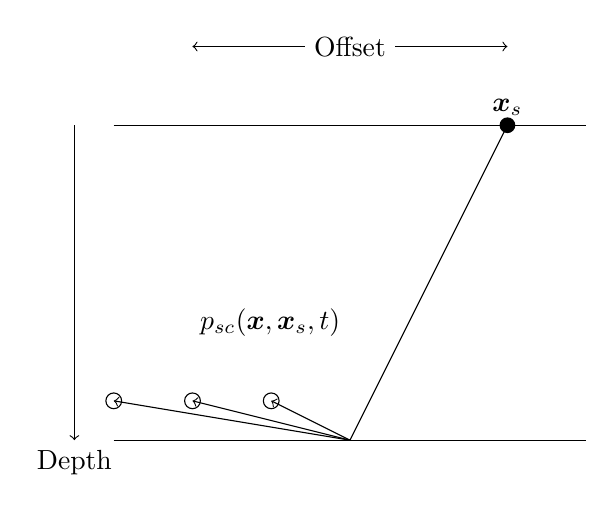
\begin{tikzpicture}[scale=1.0]
  \draw[->] (-0.5,4.0) -- (-0.5,0.0) node[below]{Depth} ;     %Draw Depth axis
  \draw[<->] (1.0,5.0) -- node[fill=white]{Offset} (5.0,5.0); %Draw offset axis 
  \draw (0.0,0.0) -- (6.0,0.0) ;  %Top boundary
  \draw (0.0,4.0) -- (6.0,4.0) ;  %Bottom boundary

  \fill (5.0,4.0) node[above]{$\xx_s$} circle (0.1) ; % Draw source

  \fill[white] (0.0,0.5) circle (0.1) ; %Draw receiver
  \draw (0.0,0.5) circle (0.1) ;
  

  \fill[white](1.0,0.5) circle (0.1) ;
  \draw (1.0,0.5) node[above]{} circle (0.1) ;

  \fill[white] (2.0,0.5) circle (0.1) ;
  \draw (2.0,0.5) circle (0.1) ;

%  \fill[white] (3.0,0.5) circle (0.1) ;
%  \draw (3.0,0.5) circle (0.1) ;

%  \fill[white] (4.0,0.5) circle (0.1) ;
%  \draw (4.0,0.5) circle (0.1) ;

  \draw[->] (3,0)-- (0.0,0.5);
  \draw[->] (3,0)-- (1.0,0.5);
  \draw[->] (3,0)-- (2.0,0.5);
  %\draw[->] (3,0)-- (3.0,0.5);
  %\draw[->] (3,0)-- (4.0,0.5);
%  \draw (3,0) +(0:0.25) arc(0:180:0.25);
%  \draw (3,0) +(80:3) arc(80:152:3);
  \draw (3.0,1.5) node[left]{$p_{sc}(\xx,\xx_s,t)$};


  \draw (5.0,4.0) -- (3.0,0.0) ;
  %\draw (3.0,0.0) -- (1.0,4.0) ;
\end{tikzpicture}
%\label{fig:si-1}
\end{figure}
\end{frame}
%-----------------------------------------
\begin{frame}{Imaging condition V}
%-----------------------------------------
\begin{figure}
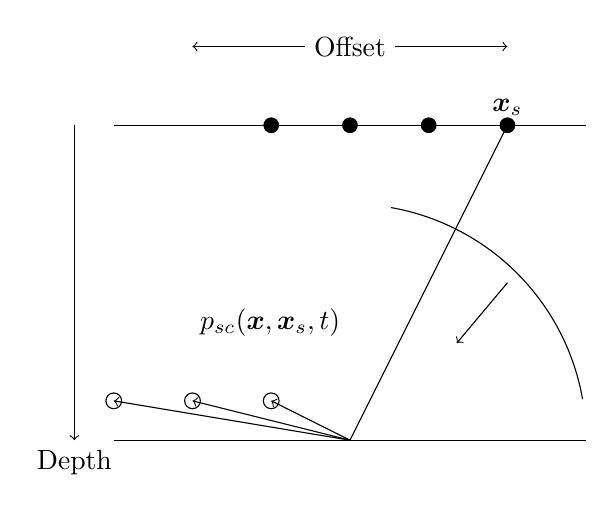
\begin{tikzpicture}[scale=1.0]
  \draw[->] (-0.5,4.0) -- (-0.5,0.0) node[below]{Depth} ;     %Draw Depth axis
  \draw[<->] (1.0,5.0) -- node[fill=white]{Offset} (5.0,5.0); %Draw offset axis 
  \draw (0.0,0.0) -- (6.0,0.0) ;  %Top boundary
  \draw (0.0,4.0) -- (6.0,4.0) ;  %Bottom boundary

  \fill (5.0,4.0) node[above]{$\xx_s$} circle (0.1) ; % Draw source
  \fill (4.0,4.0) node[above]{} circle (0.1) ; % Draw source
  \fill (3.0,4.0) node[above]{} circle (0.1) ; % Draw source
  \fill (2.0,4.0) node[above]{} circle (0.1) ; % Draw source

  \fill[white] (0.0,0.5) circle (0.1) ; %Draw receiver
  \draw (0.0,0.5) circle (0.1) ;
  

  \fill[white](1.0,0.5) circle (0.1) ;
  \draw (1.0,0.5) node[above]{} circle (0.1) ;

  \fill[white] (2.0,0.5) circle (0.1) ;
  \draw (2.0,0.5) circle (0.1) ;

%  \fill[white] (3.0,0.5) circle (0.1) ;
%  \draw (3.0,0.5) circle (0.1) ;

%  \fill[white] (4.0,0.5) circle (0.1) ;
%  \draw (4.0,0.5) circle (0.1) ;

  \draw[->] (3,0)-- (0.0,0.5);
  \draw[->] (3,0)-- (1.0,0.5);
  \draw[->] (3,0)-- (2.0,0.5);
%  \draw[->] (3,0)-- (3.0,0.5);
%  \draw[->] (3,0)-- (4.0,0.5);
%  \draw (3,0) +(0:0.25) arc(0:180:0.25);
%  \draw (3,0) +(80:3) arc(80:152:3);
  \draw (3.0,1.5) node[left]{$p_{sc}(\xx,\xx_s,t)$};
\draw (3,0) +(80:3) arc(80:10:3);

  \draw[->] (5,2)-- +(230:1);

  \draw (5.0,4.0) -- (3.0,0.0) ;
  %\draw (3.0,0.0) -- (1.0,4.0) ;
\end{tikzpicture}
%\label{fig:si-1}
\end{figure}
\end{frame}
%-----------------------------------------
\begin{frame}{Imaging condition VI}
%-----------------------------------------
\begin{figure}
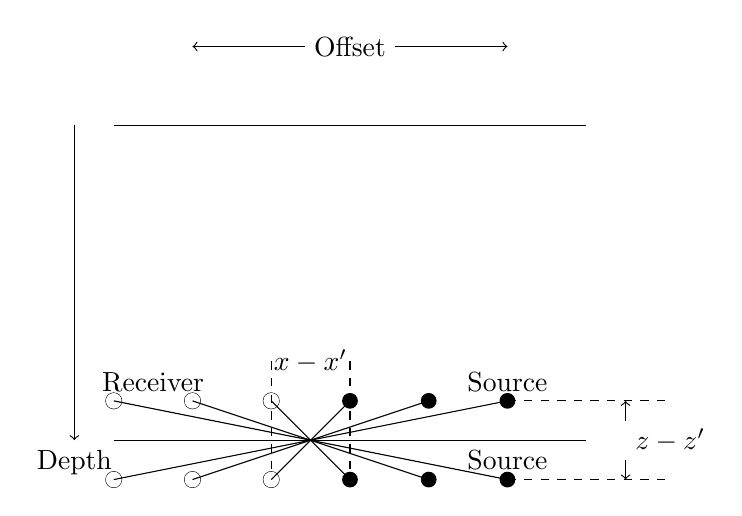
\begin{tikzpicture}[scale=1.0]
   \draw[->] (-0.5,4.0) -- (-0.5,0.0) node[below]{Depth} ;      %Depth axis 
   \draw[<->] (1.0,5.0) -- node[fill=white]{Offset} (5.0,5.0);  %Offset axis  
  \draw (0.0,4.0) -- (6.0,4.0) ;                               % Boundary at top
  \draw (0.0,0.0) -- (6.0,0.0) ;                               % Boundary at depth

  \fill (3.0,0.5) node[above]{} circle (0.1) ;           % Draw source
  \fill (4.0,0.5) node[above]{} circle (0.1) ;           % Draw source
  \fill (5.0,0.5) node[above]{Source} circle (0.1) ;     % Draw source text

  \draw (2.0,0.5) circle (0.1) ;             %Draw receiver
  \fill[white] (2.0,0.5) circle (0.1) ;

  \draw (1.0,0.5) circle (0.1) ;             %Draw receiver
  \fill[white] (1.0,0.5) circle (0.1) ;

  \draw (0.0,0.5) circle (0.1) ;             %Draw receiver
  \fill[white] (0.0,0.5) circle (0.1) ;
  \draw (0.5,0.5) node[above]{Receiver} ;    %Draw receiver text 

  \draw (3.0,0.5) -- (2.5,0.0);              % Draw ray from source to midpoint
  \draw (4.0,0.5) -- (2.5,0.0);              % Draw ray from source to midpoint
  \draw (5.0,0.5) -- (2.5,0.0);              % Draw ray from source to midpoint

  \draw (2.0,0.5) -- (2.5,0.0);              % Draw ray from receiver to midpoint
  \draw (1.0,0.5) -- (2.5,0.0);              % Draw ray from receiver to midpoint
  \draw (0.0,0.5) -- (2.5,0.0);              % Draw ray from receiver to midpoint

  \draw[dashed] (2.0,1.0) -- (2.0,-0.5);     %Draw vertical dashed line
  \draw[dashed] (3.0,1.0) -- (3.0,-0.5);     %Draw vertical dashed line
  \draw (2.5,1.0) node {$x-x'$};           % Draw equation
  \draw[dashed] (5.0,0.5) -- (7.0,0.5);     %Draw vertical dashed line
  \draw[dashed] (5.0,-0.5) -- (7.0,-0.5);     %Draw vertical dashed line
  \draw (6.5,0.0) node[right]{$z-z'$};           % Draw equation
  \draw[->] (6.5,0.25) -- (6.5,0.5);
  \draw[->] (6.5,-0.25) -- (6.5,-0.5);



  \fill (3.0,-0.5) node[above]{} circle (0.1) ;           % Draw source
  \fill (4.0,-0.5) node[above]{} circle (0.1) ;           % Draw source
  \fill (5.0,-0.5) node[above]{Source} circle (0.1) ;     % Draw source text

  \draw (2.0,-0.5) circle (0.1) ;             %Draw receiver
  \fill[white] (2.0,-0.5) circle (0.1) ;

  \draw (1.0,-0.5) circle (0.1) ;             %Draw receiver
  \fill[white] (1.0,-0.5) circle (0.1) ;

  \draw (0.0,-0.5) circle (0.1) ;             %Draw receiver
  \fill[white] (0.0,-0.5) circle (0.1) ;
  %\draw (0.5,0.5) node[above]{Receiver} ;    %Draw receiver text 

  \draw (3.0,-0.5) -- (2.5,0.0);              % Draw ray from source to midpoint
  \draw (4.0,-0.5) -- (2.5,0.0);              % Draw ray from source to midpoint
  \draw (5.0,-0.5) -- (2.5,0.0);              % Draw ray from source to midpoint

  \draw (2.0,-0.5) -- (2.5,0.0);              % Draw ray from receiver to midpoint
  \draw (1.0,-0.5) -- (2.5,0.0);              % Draw ray from receiver to midpoint
  \draw (0.0,-0.5) -- (2.5,0.0);              % Draw ray from receiver to midpoint
\end{tikzpicture}
\end{figure}

$x-x'$: Horizontal offset \\
$z-z'$: Vertical offset 
\end{frame}
%-----------------------------------------
\begin{frame}{New Imaging condition}
%-----------------------------------------
Redatumed scattered wavefield: 
\begin{eqnarray}
  p_{sc}(\xx,\xx',t)*s(-t) 
   \approx 2\sum_{\xx_s}\sum_{\tau}\d_{z_s} p_0(\xx,\xx_s,t+\tau)p_{sc}(\xx',\xx_s,\tau)\nonumber\\ 
                       \nonumber
\end{eqnarray}
\begin{itemize}
\item $p_0(\xx.\xx_s,t)$: Forward simulated wavefield
\item $p_sc(\xx',\xx_s)$: Back propagated scattered wavefield (data)
\item $s(t)$: Source signature
\end{itemize}
(Oristaglio, 1989\cite{Oristaglio1989} and Wapenaar, 2007 \cite{Wapenaar2007}).

\vspace{1cm}
New imaging condition:
\begin{eqnarray}
  r(\xx,\xx')\nonumber & = & 
  p_{sc}(\xx,\xx',t)*s(-t)|_{t=0} =\nonumber\\ 
   &\approx& 2\sum_{\xx_s}\sum_{\tau}\d_{z_s} p_0(\xx,\xx_s,\tau)p_{sc}(\xx',\xx_s,\tau)\nonumber\\ 
                       \nonumber
\end{eqnarray}
\end{frame}
%-----------------------------------------
\begin{frame}{Classical Imaging condition}
%-----------------------------------------
For $\xx'=\xx$ and by ignoring $\partial_z$ this is the classical imaging condition (Claerbout, 1971) \cite{Claerbout1971}
\begin{eqnarray}
  r_{c}(\xx) =
    \sum_{\xx_s}\sum_{\tau}p_0(\xx,\xx_s,\tau)p_{sc}(\xx,\xx_s,\tau)\nonumber\\ 
                                                 \nonumber
\end{eqnarray}

Ignoring $\partial_z$ implies an unfocused image with 
less than optimal resolution and incorrect amplitudes.
\end{frame}
%-----------------------------------------
\begin{frame}{Numerical examples}
%-----------------------------------------
\begin{figure}
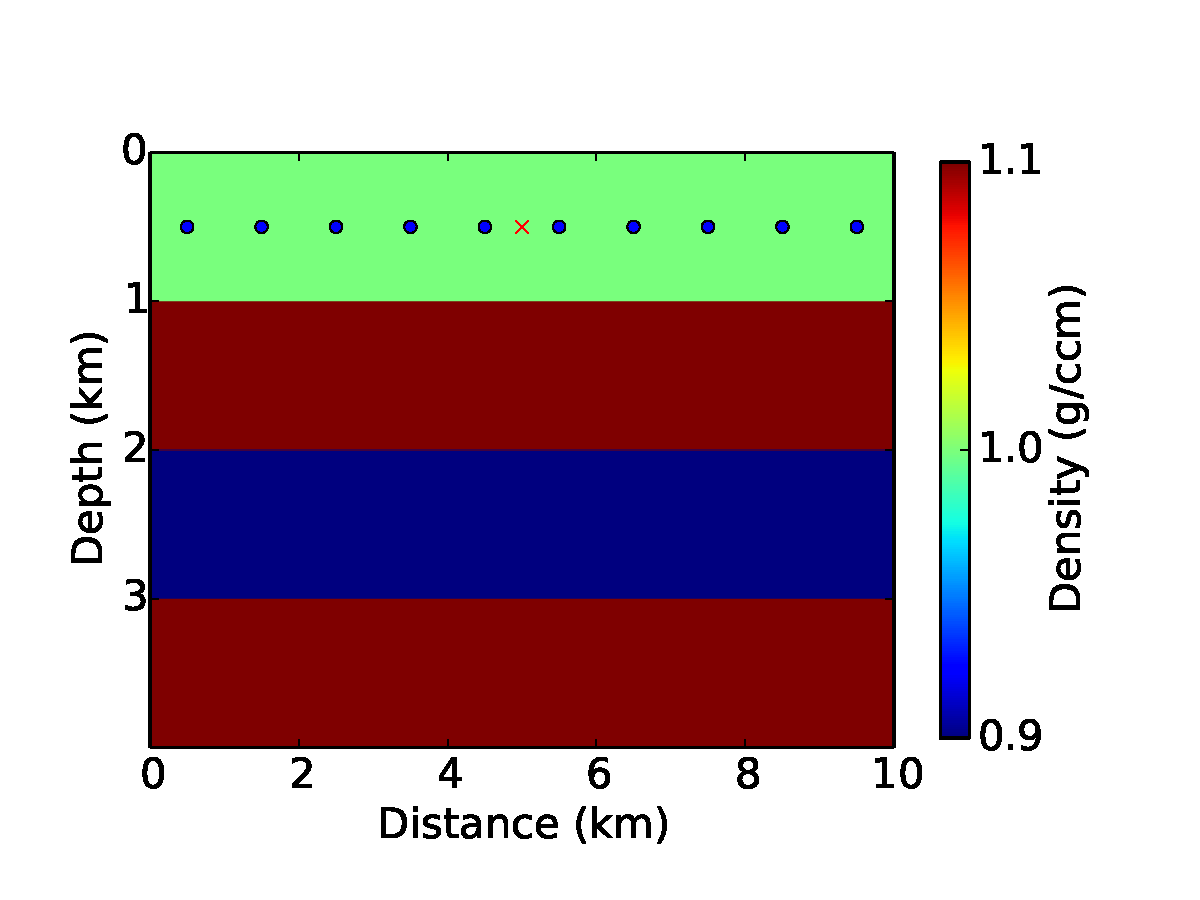
\epsfig{file=Fig/case-3-rho,width=5cm}
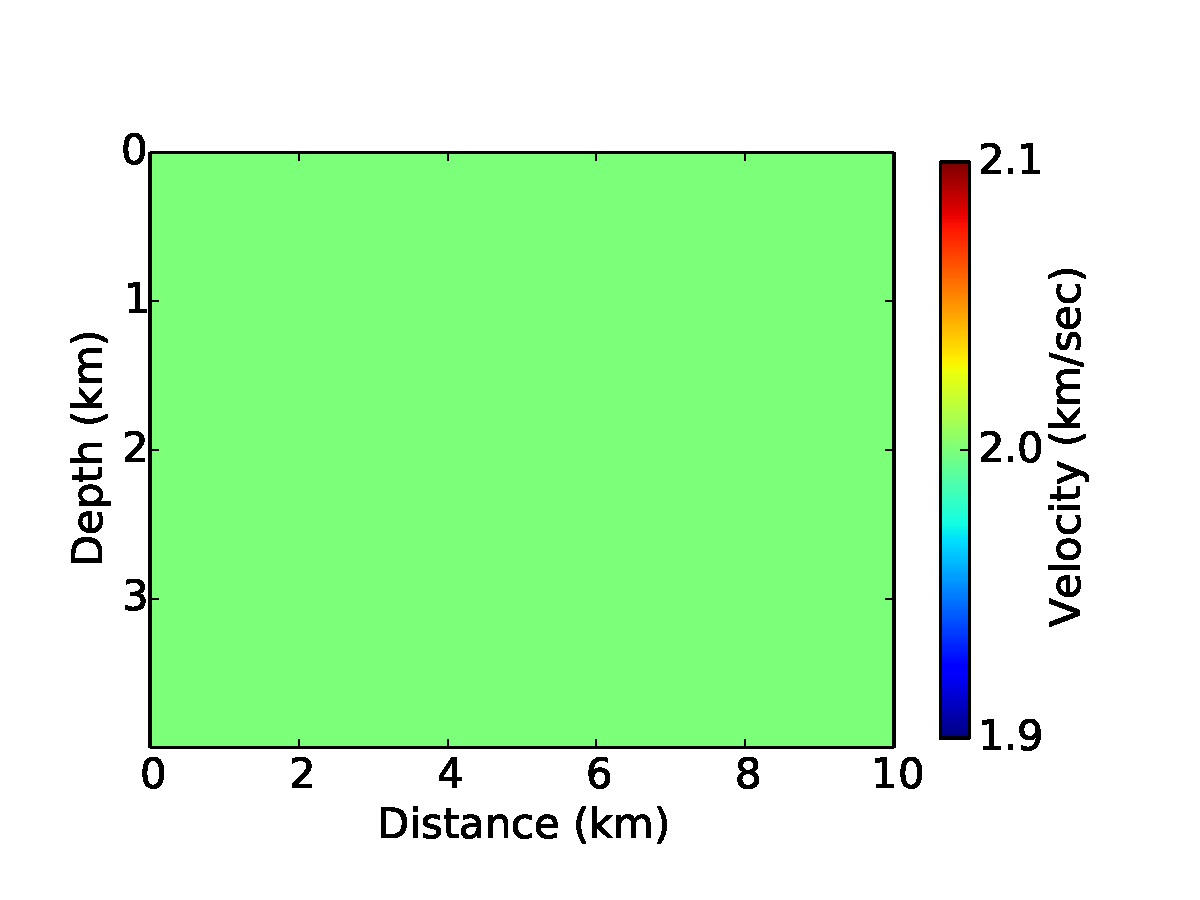
\epsfig{file=Fig/case-3-vp,width=5cm}
\end{figure}
\end{frame}
%-----------------------------------------
\begin{frame}{Numerical examples}
%-----------------------------------------
\begin{figure}
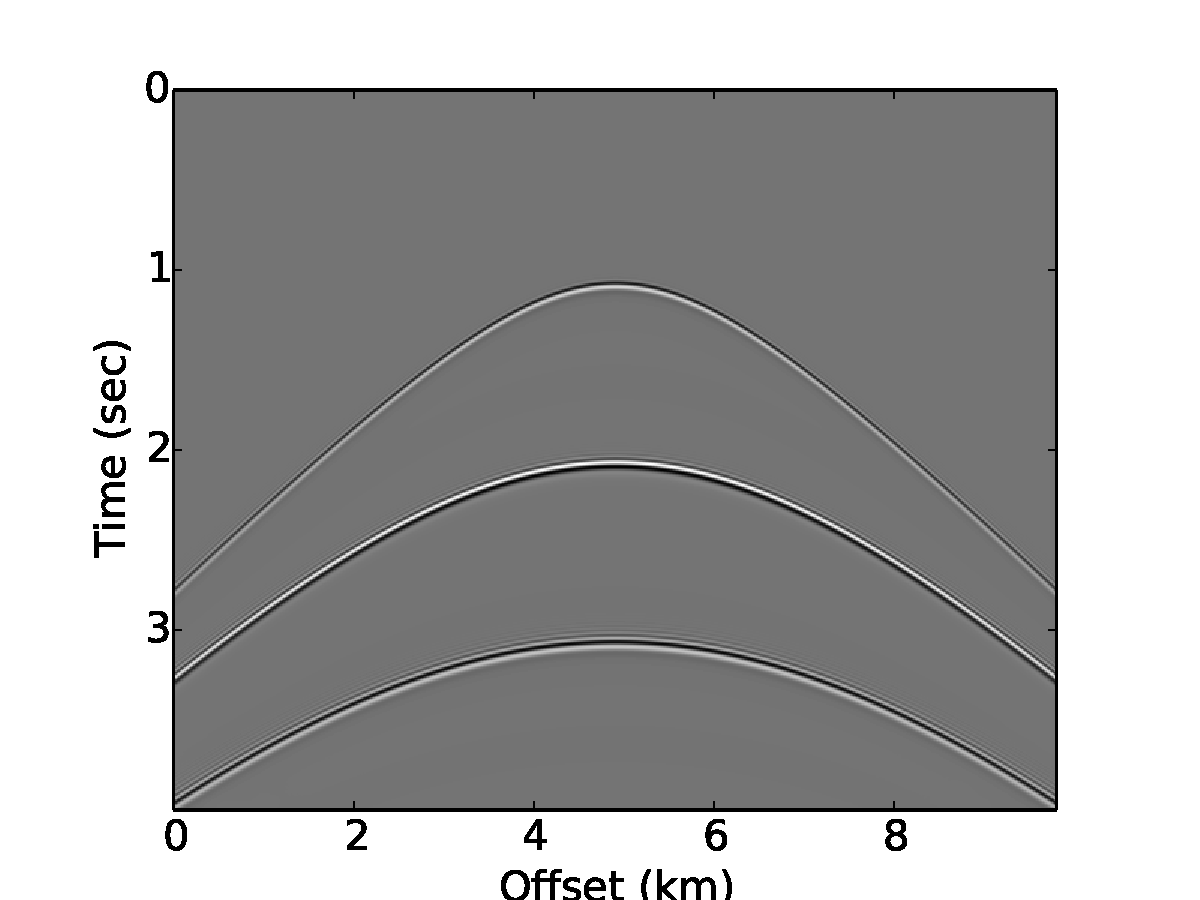
\epsfig{file=Fig/case-3-data-scatter,width=10cm}
\end{figure}
\end{frame}
%------------------------------------------------------
\begin{frame}{Numerical examples}
%------------------------------------------------------
Common image point gather (CIP) in the center of the model
Classical imaging condition: 
\begin{figure}
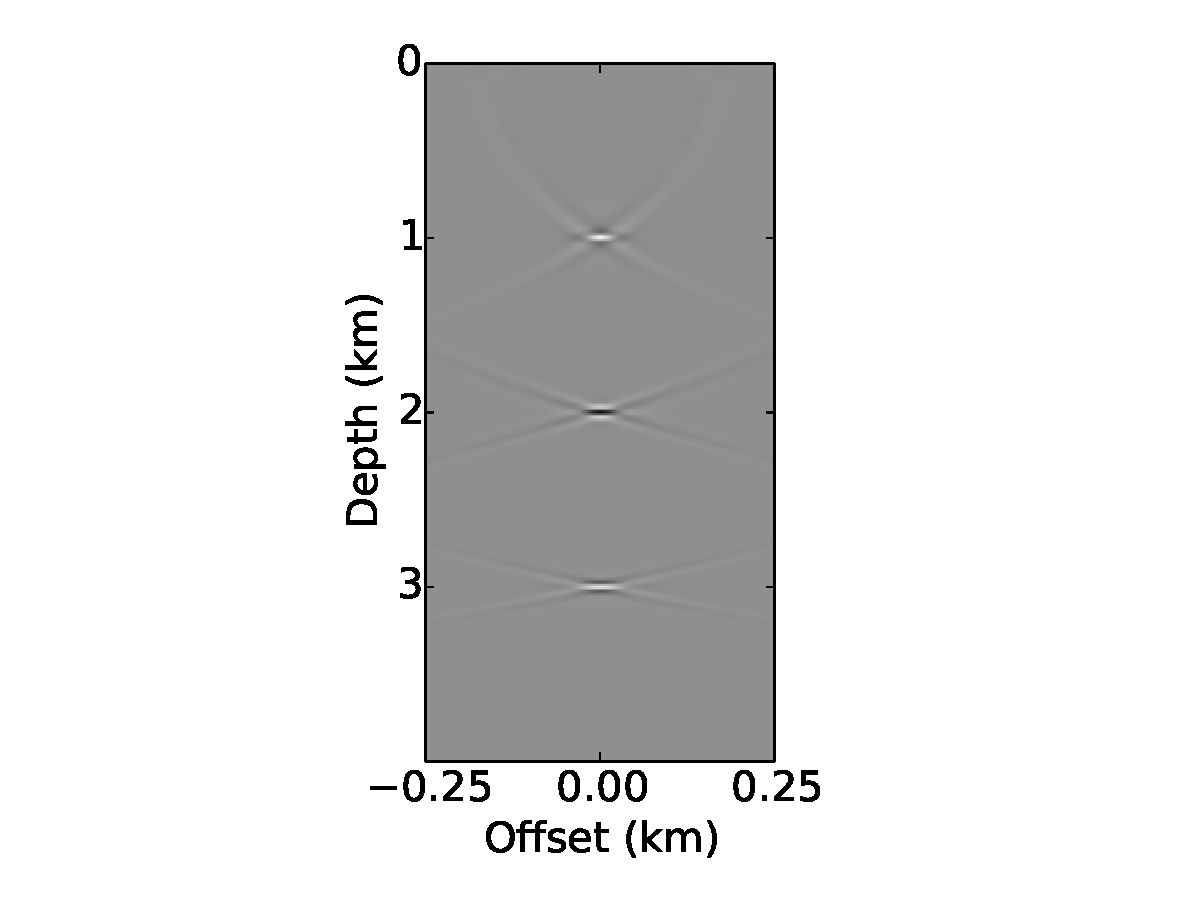
\epsfig{file=Fig/case-1-cig,width=9cm}
\end{figure}
\end{frame}
%------------------------------------------------------
\begin{frame}{Numerical examples}
%------------------------------------------------------
Horizontal profile through reflector at 1000m depth
\begin{figure}
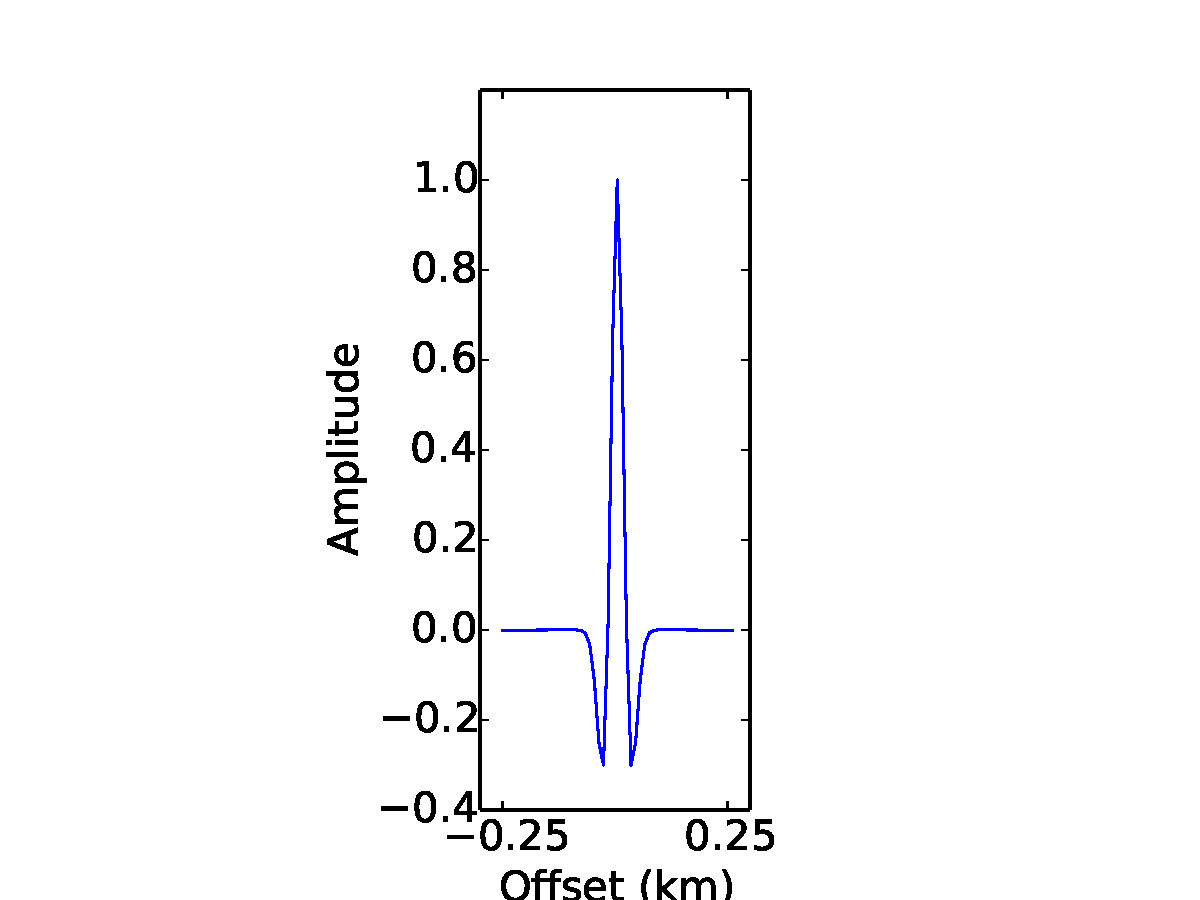
\epsfig{file=Fig/case-1-cig-h,width=9cm}
\end{figure}
\end{frame}
%------------------------------------------------------
\begin{frame}{Numerical examples}
%------------------------------------------------------
Common image point gather (CIP) in the center of the model.\\
New imaging condition: 
\begin{figure}
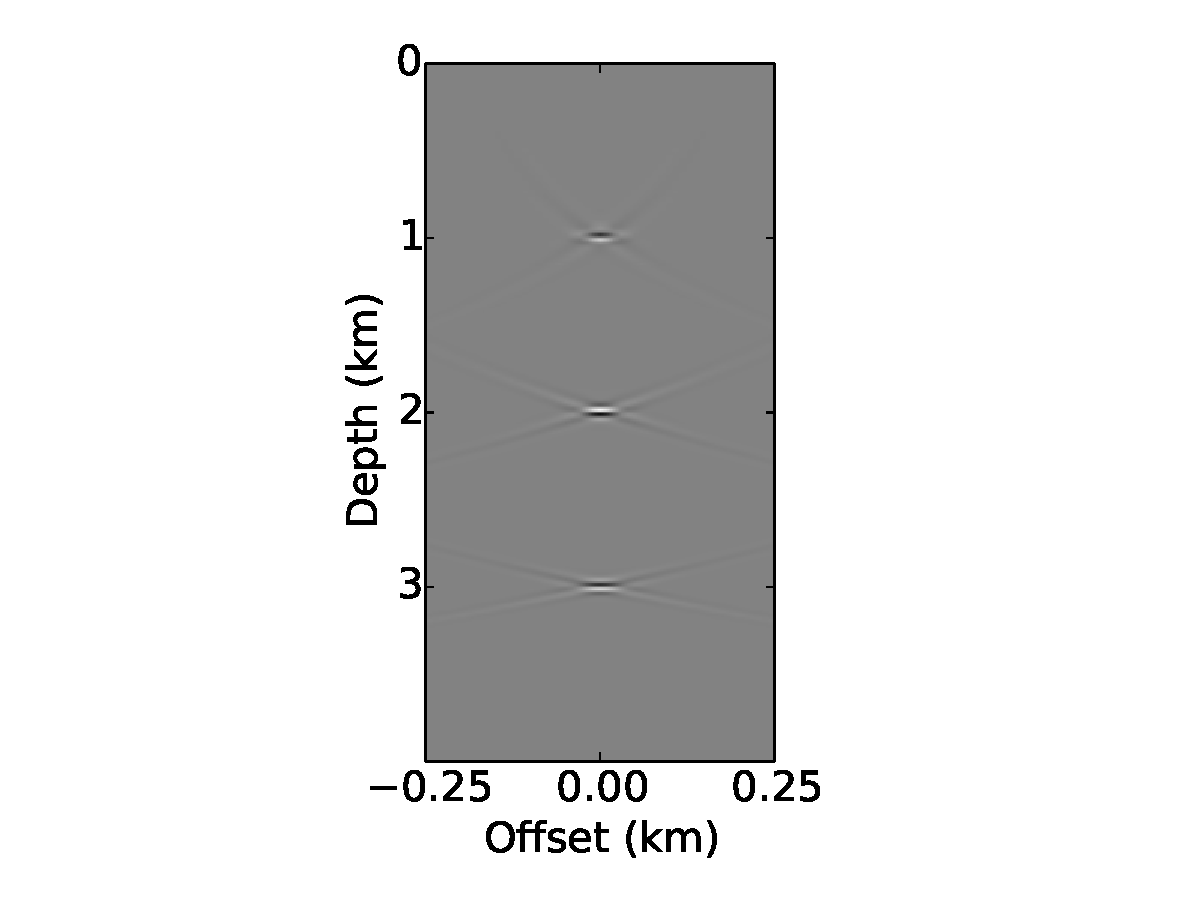
\epsfig{file=Fig/case-2-cig,width=9cm}
\end{figure}
\end{frame}
%------------------------------------------------------
\begin{frame}{Numerical examples}
%------------------------------------------------------
Horizontal profile through reflector at 1000m depth
\begin{figure}
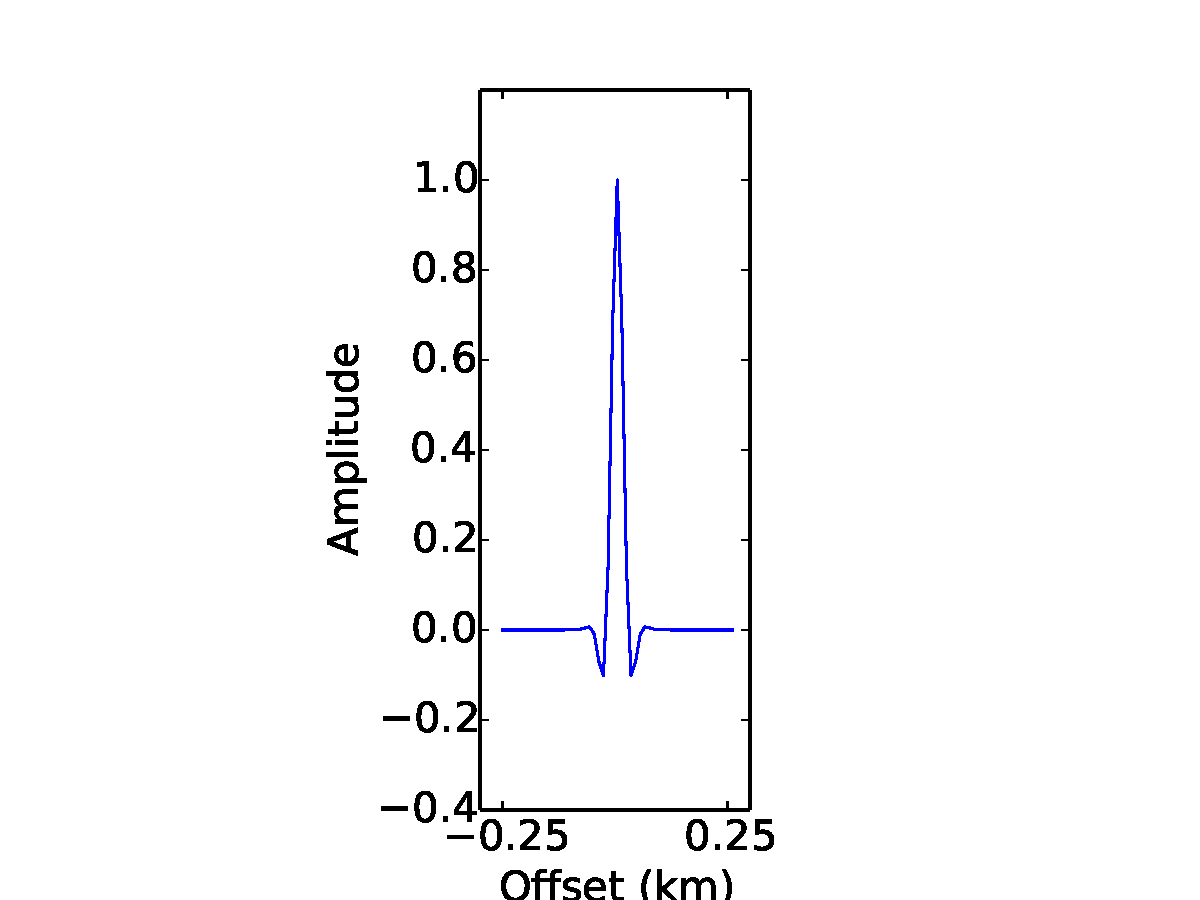
\epsfig{file=Fig/case-2-cig-h,width=9cm}
\end{figure}
\end{frame}
%------------------------------------------------------
\begin{frame}{Numerical example}
%------------------------------------------------------
Conventional imaging condition:
\begin{figure}
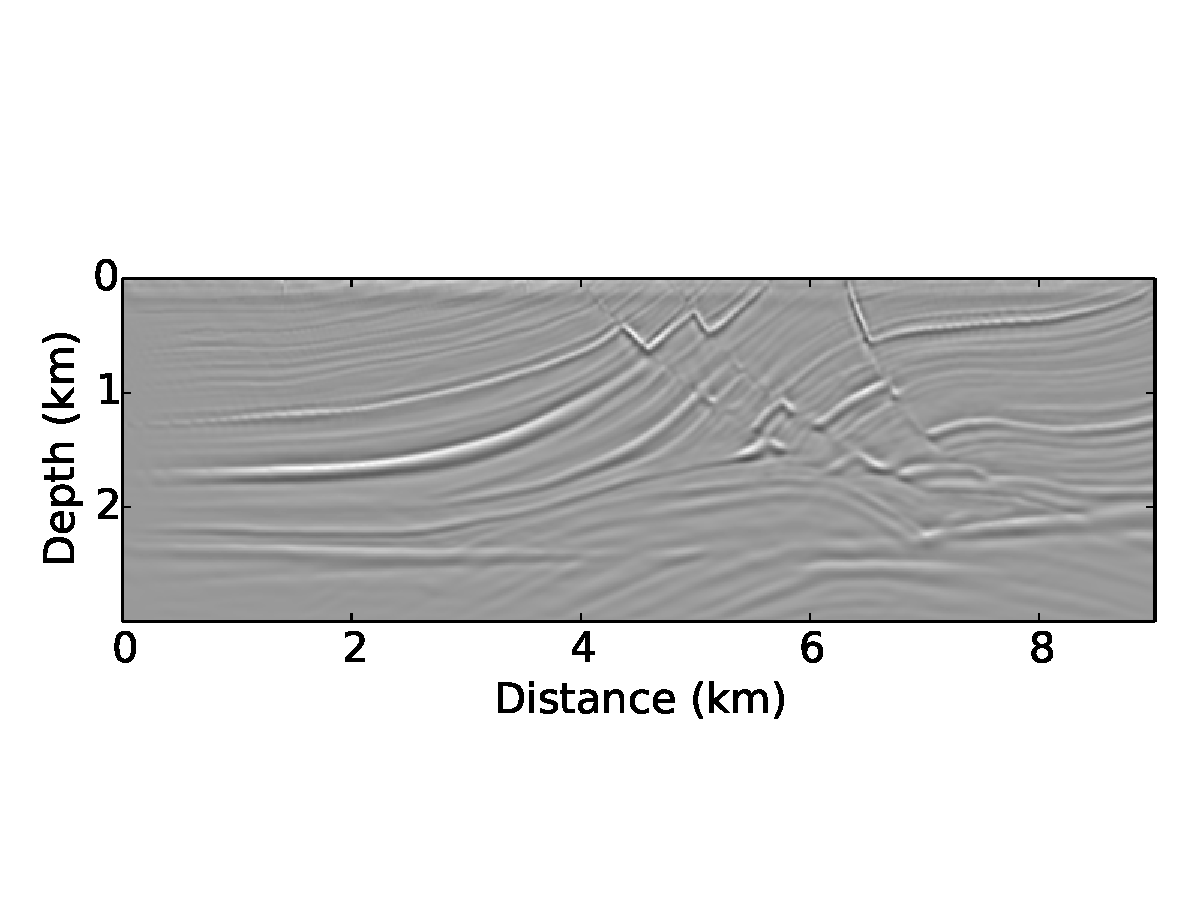
\epsfig{file=Fig/case-4-stack,width=10cm}
\end{figure}
\end{frame}
%------------------------------------------------------
\begin{frame}{Numerical example}
%------------------------------------------------------
New imaging condition:
\begin{figure}
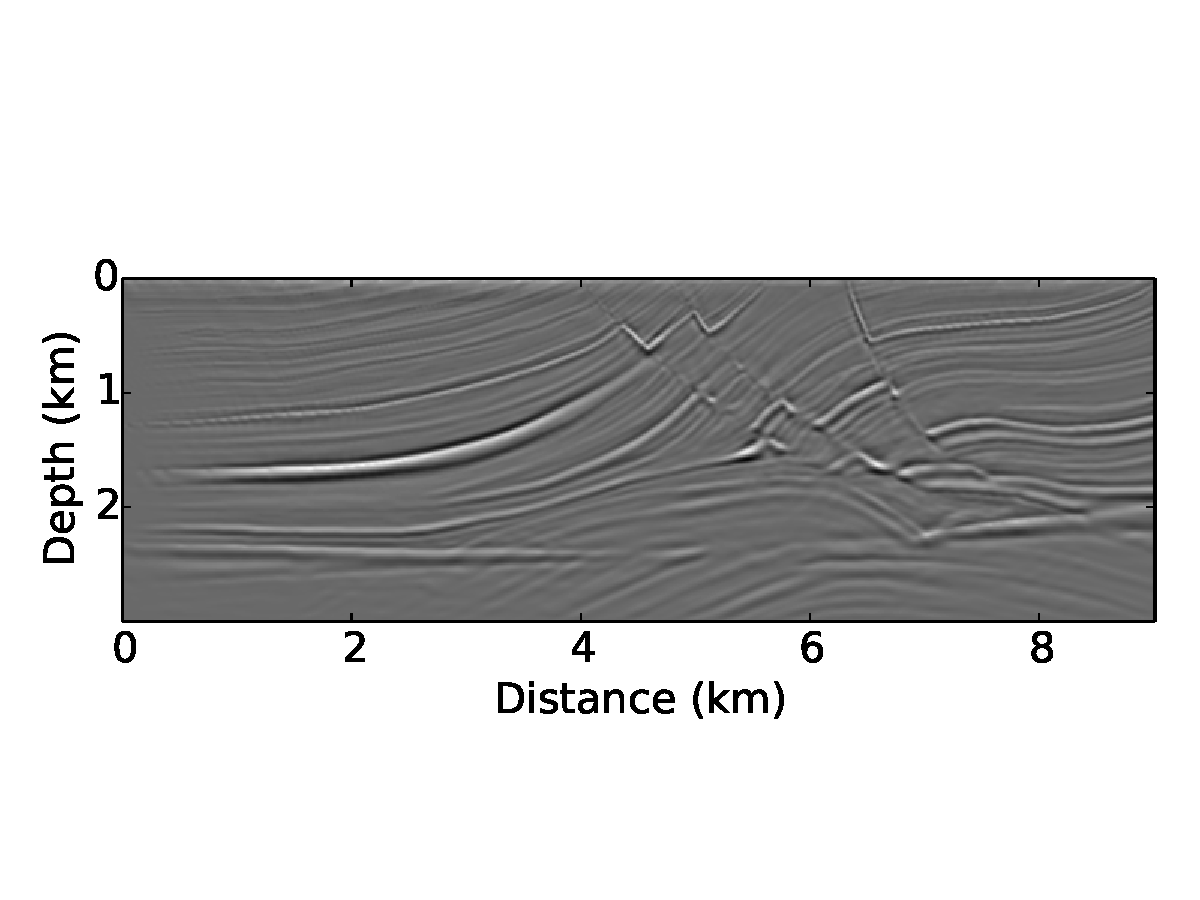
\epsfig{file=Fig/case-5-stack,width=10cm}
\end{figure}
\end{frame}
%------------------------------------------------------
\begin{frame}{Numerical example}
%------------------------------------------------------
Conventional imaging condition:
\begin{figure}
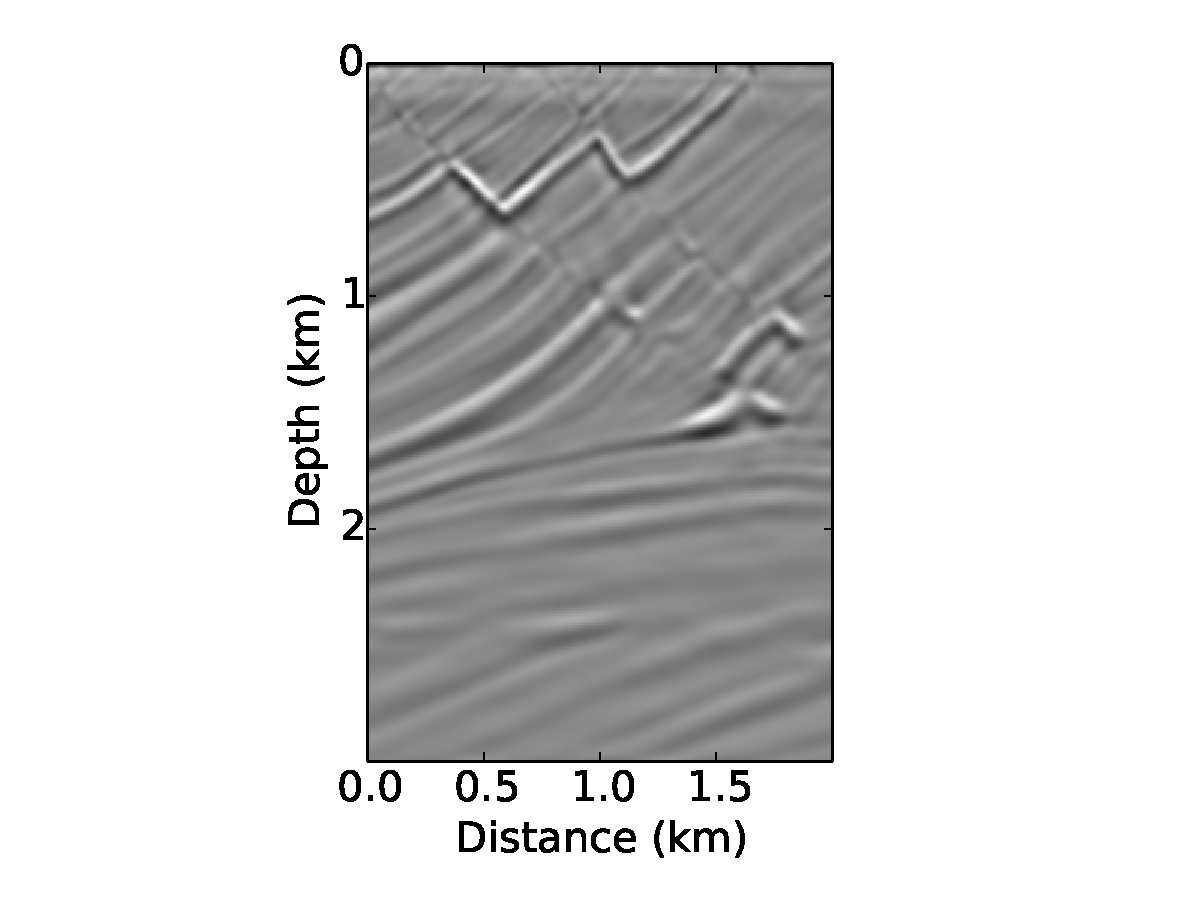
\epsfig{file=Fig/case-4-stack-zoom,width=9cm}
\end{figure}
\end{frame}
%------------------------------------------------------
\begin{frame}{Numerical example}
%------------------------------------------------------
New imaging condition:
\begin{figure}
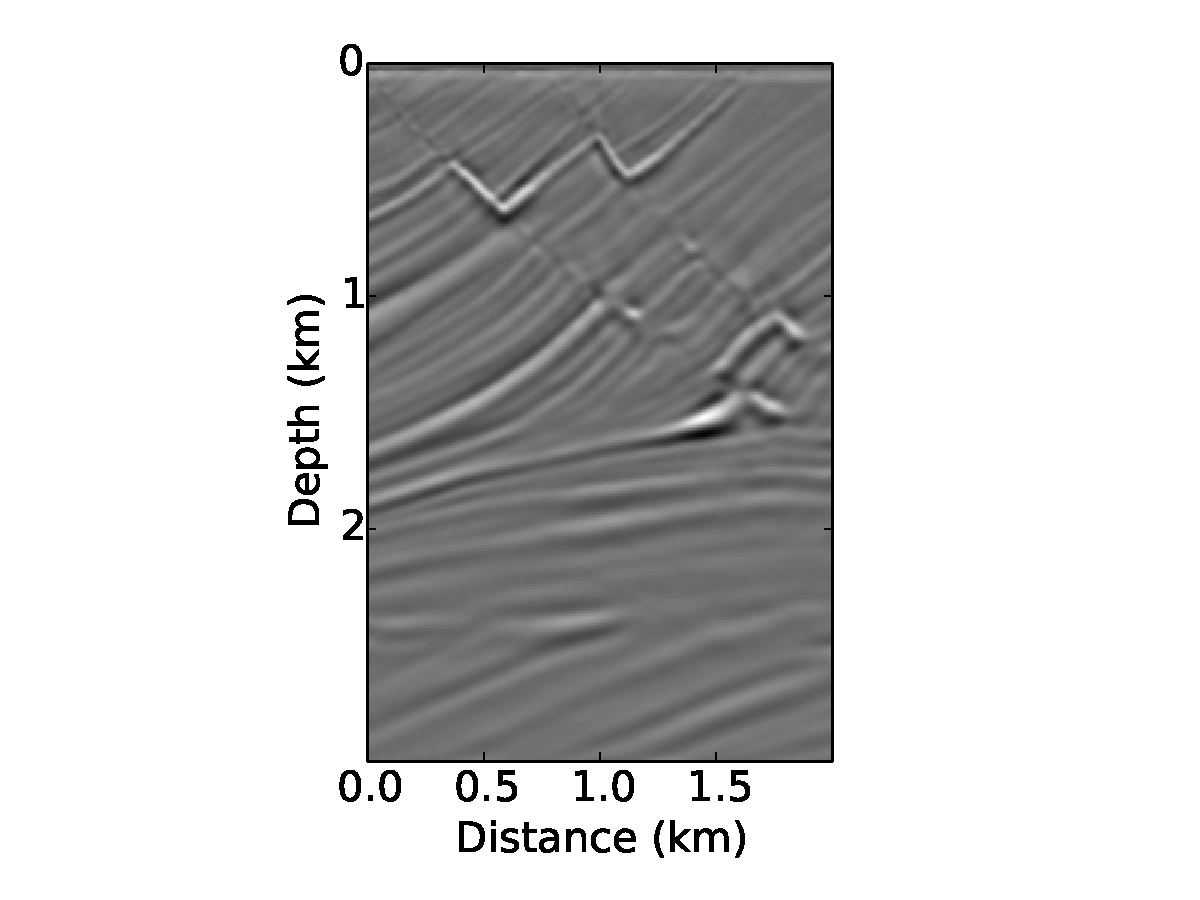
\epsfig{file=Fig/case-5-stack-zoom,width=9cm}
\end{figure}
\end{frame}
%------------------------------------------------------
\begin{frame}{Numerical example}
%------------------------------------------------------
From reflectivity to plane wave reflection coefficient
\begin{eqnarray}
  \partial_z r(\xx,\xx',t) & = & 
   2\sum_{\xx_s}\sum_{\tau}\d^2_{z_s} p_0(\xx,\xx_s,\tau+t)p_{sc}(\xx',\xx_s,\tau)
\end{eqnarray}
Plane wave reflection coefficient by mapping to $p-\tau$ (deBruin 1991\cite{Bruin1990}) 

\vspace{1cm}
Conventional approach:
\begin{eqnarray}
  r(\xx,\xx',t) & = & 
   2\sum_{\xx_s}\sum_{\tau}p_0(\xx,\xx_s,\tau+t)p_{sc}(\xx',\xx_s,\tau)
\end{eqnarray}
Plane wave reflection coefficient by mapping to $p-\tau$ (deBruin 1991\cite{Bruin1990}) 

\end{frame}
%------------------------------------------------------
\begin{frame}{Numerical example}
%------------------------------------------------------
$p$-gather at the center of the model
\begin{figure}
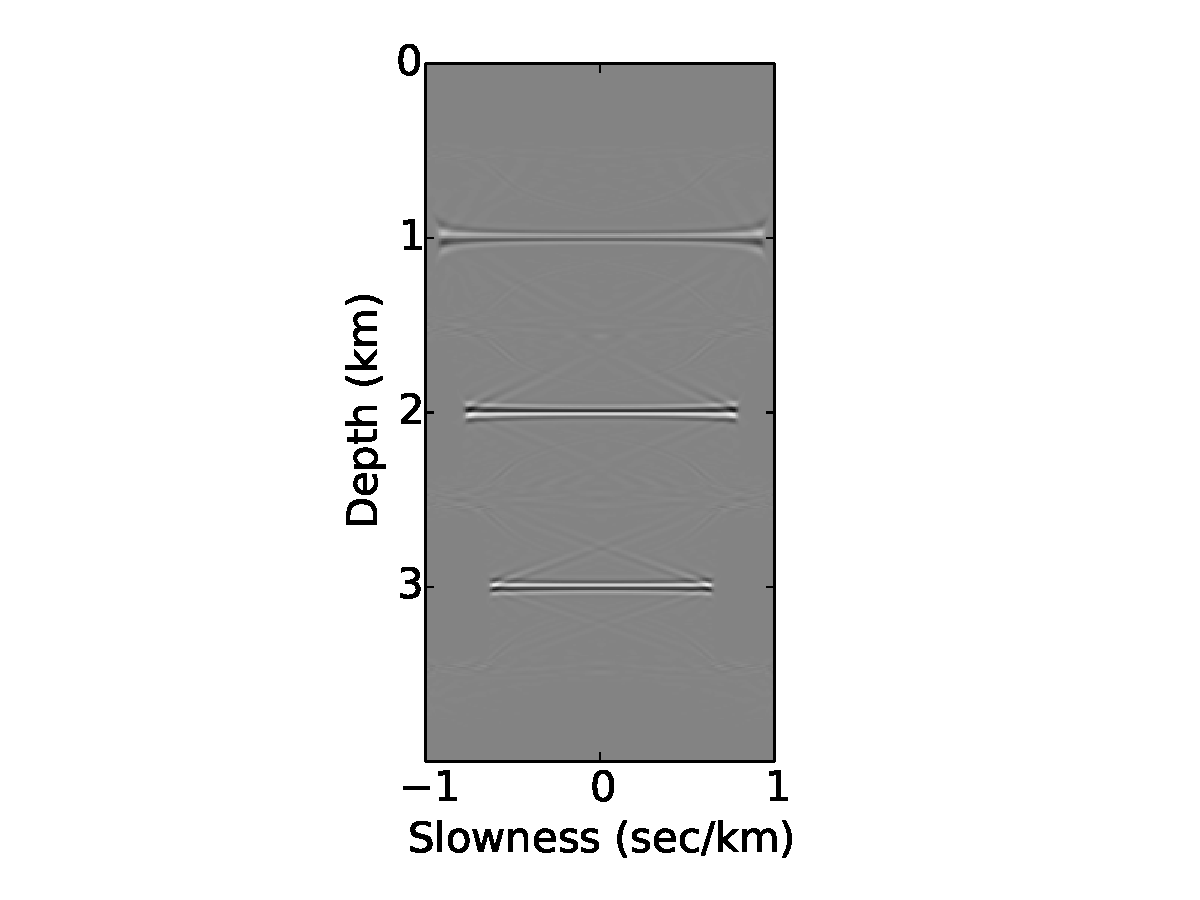
\epsfig{file=Fig/case-3-cag,width=10cm}
\end{figure}
\end{frame}
%------------------------------------------------------
\begin{frame}{Numerical example}
%------------------------------------------------------
Amplitude picks along $p$-gather
\begin{figure}
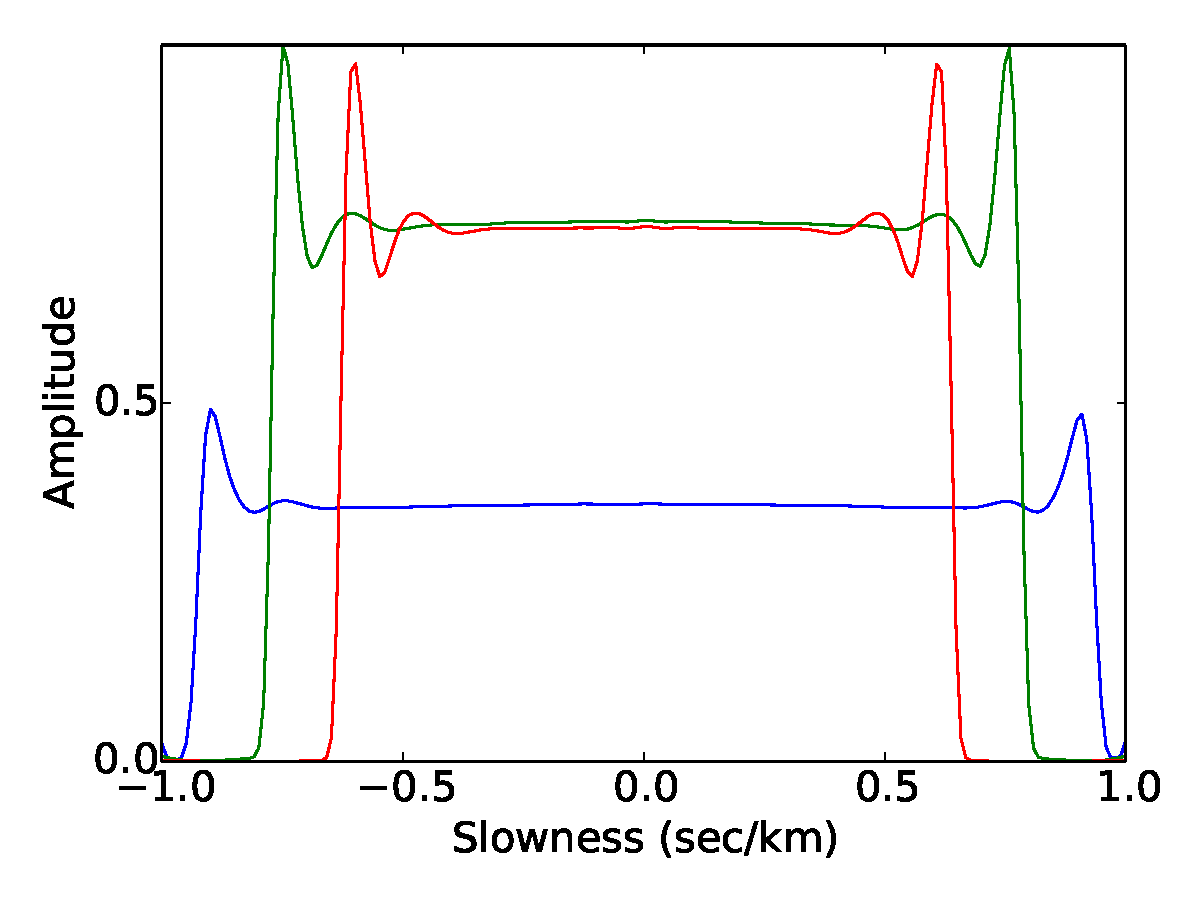
\epsfig{file=Fig/case-3-pick,width=10cm}
\end{figure}
\end{frame}
%------------------------------------------------------
\begin{frame}{Numerical example}
%------------------------------------------------------
Conventional approach:
\begin{figure}
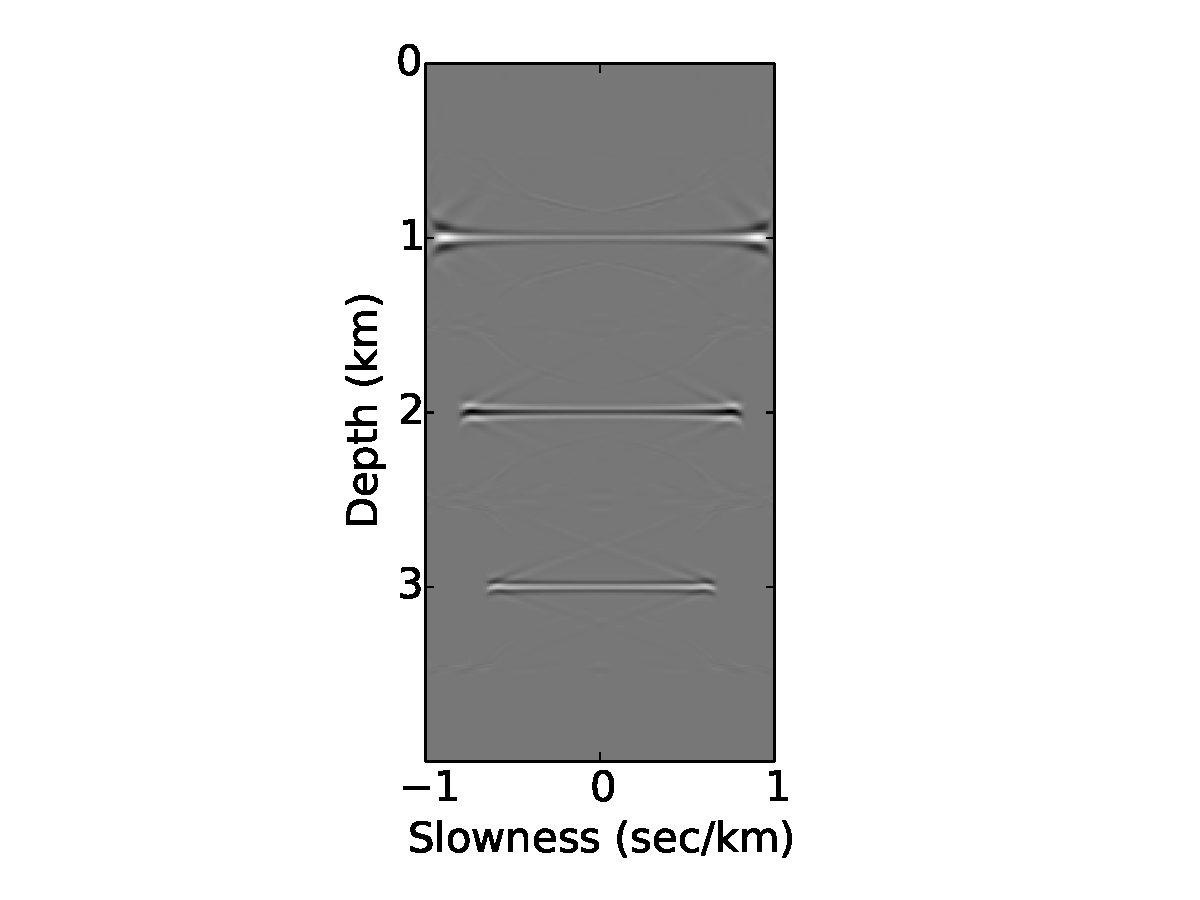
\epsfig{file=Fig/case-1-cag,width=10cm}
\end{figure}
\end{frame}
%------------------------------------------------------
\begin{frame}{Numerical example}
%------------------------------------------------------
Amplitude picks along $p$-gather
\begin{figure}
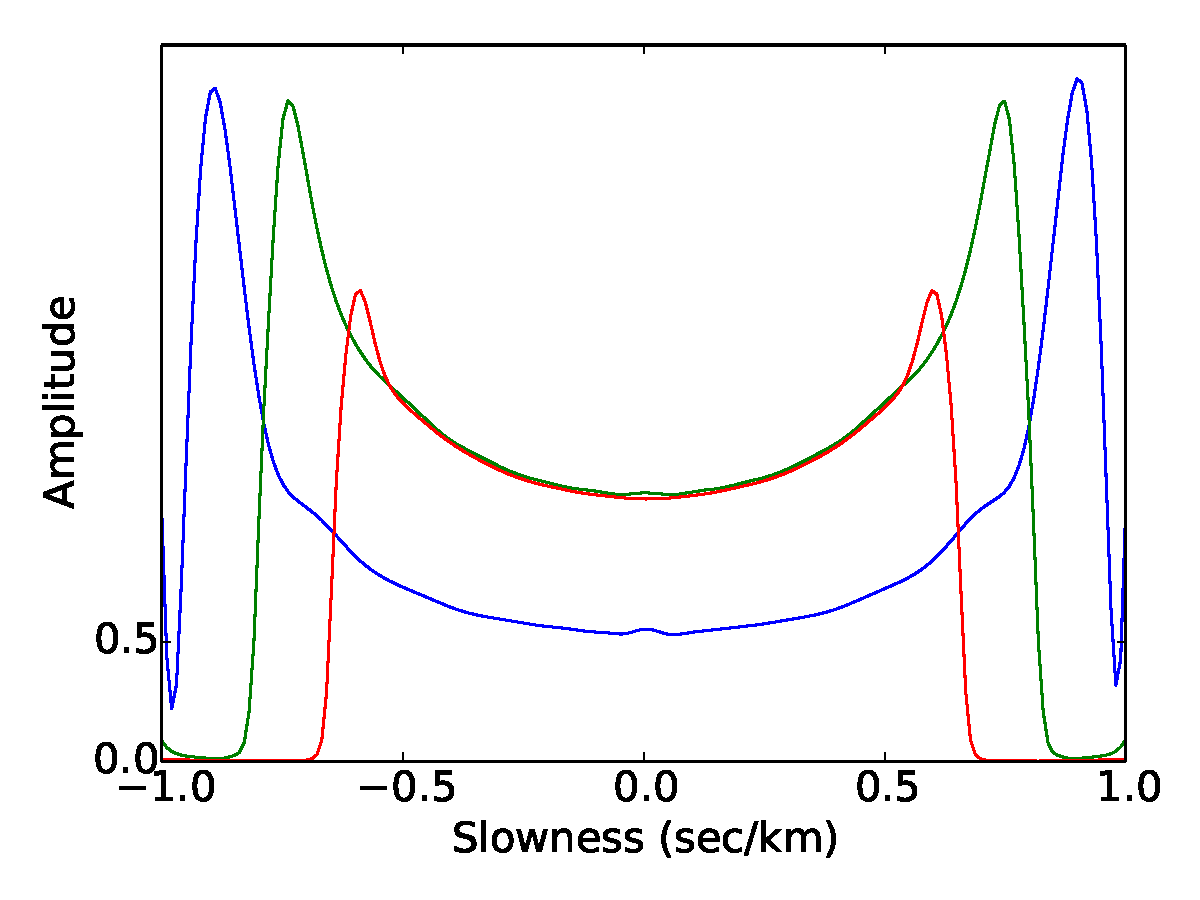
\epsfig{file=Fig/case-1-pick,width=10cm}
\end{figure}
\end{frame}
%-----------------------------------------
\begin{frame}{Conclusions}
%-----------------------------------------
Simple (trivial) modification of the classical
imaging condition for Reverse-time migration gives
\begin{itemize}
  \item Better resolution
  \item Reflectivity with correct angle behavior
\end{itemize}
\end{frame}
%-----------------------------------------
\begin{frame}{Bibliography}
%-----------------------------------------
\bibliographystyle{plain}
\bibliography{references}
\end{frame}

\end{document}

